Titelblatt

Abstract

Pathfinding-Algorithmen sind Programmablaufe, welche in der Wirtschaft
in vielen Anwendun- ¨ gen vorkommen, wie zum Beispiel Video Spielen,
Simulationen oder der Automobilindustrie. Diese Berufsmaturitatsarbeit
implementiert mehrere solcher Pathfinding-Algorithmen in einer ¨
interaktiven JavaScript-Webapplikation und vergleicht sie auf mehrere
Eigenschaften miteinander. Der Vergleich ist visuell dargestellt und vom
Nutzer durch Parameter in der Benutzeroberflache anpassbar. Ausgew ¨
ahlt wurden daf ¨ ur die drei Pathfinder: A*, BestFirstFinder und ¨
BreadthFirstFinder. Die Webapplikation ist freie Software und unter
https://bma.fuerbringer.info zuganglich.

\textbf{Einleitung}

\textbf{Fragestellungen/Ziel der Arbeit}

Algorithmen sind überall in unserem Leben zu finden, selbst dort, wo wir
sie nicht erwarten: In der Natur, im Weltraum, oder in der Biologie. Da
das Autorenteam dieser Berufsmaturitätsarbeit sehr technisch
interessiert ist wird in dieser Arbeit eine bedeutende Klasse der
Algorithmen ausgewertet. Das vorgegebene Oberthema ist ``Mobilität''.
Aufgrund des gegebenen Thema haben wir uns für die Zweidimensionalen
Matrix Pathfinding-Algorithmus entschieden. Einer der bekanntesten
Algorithmen in diesem Themenbereich ist der Dijkstra A* (,,A-Star")
Algorithmus. Es ist allgemein bekannt er sei der effizienteste.

Die merkmale von Algorithmen sind in unserer Zeit extrem wichtig, sie
definiert die Vor- und Nachteile von Algorithmen bei ihrer Ausführung.
Die Merkmale definiert Aufwand der Rechenleistung, Zeit die benötigt
wird für das Ergebnis, Tiefe der Suche nach der besten oder optimalsten
Lösung. Intelligente Systeme wie z.B. Künstliche Intelligenz,
maschinelles Lernen oder der neuesten Deep-learning Technologie bauen
auf der Algorithmentechnologie auf.

Durch Vergleiche dreier Pathfinding Algorithmen wollen wir herausfinden,
welcher Algorithmus in welchen Situationen am effizientesten ist. Die
Drei Algorithmen sind: A*, BestFirst und BreadthFirst. Diese drei wurden
vom Autorenteam ausgewählt, da im bereits bestehenden Produkt
Unterschiede in der Ausführung und Pfadsuche sichtbar war.

Falls einer der drei Algorithmen ein anderen Weg wählt, wollen wir den
Grund dieser Entscheidung Herausfinden. Bei einem anderem Weg werden
andere Rechenoperationen ausgeführt, es kann sein, dass der beste weg
zehnmal mehr Operationen benötigte, um nur wenig effizienter zu sein.
Diese Arbeit möchten herausfinden wie das Verhältnis von aufwand zu
Effizienz bei den drei Algorithmen ist.{]}

Unsere Vermutung hinsichtlich unseren Fragestellungen ist, dass die
Algorithmen aus einem Uralgorithmus stammen und so technisch
weiterentwickelt wurden und das der Dijkstra A* (,,A-Star") in den
meisten Situationen der effizienteste Pathfinding Algorithmus ist.
{[}https://stackoverflow.com/a/9515734

\textbf{Vorgehen/Methoden}

Wir möchten erklären was Pathfinding-Algorithmen sind, was sie definiert
und wie sie ablaufen. Um dies besser zu visualisieren und die Pathfinder
zu vergleichen, wird im Rahmen dieser Berufsmaturitätsarbeit ein
technisches Produkt weiterentwickelt.

Das bestehende produkt ist hier zu finden:
http://qiao.github.io/PathFinding.js/visual/

Folgende Features wurden Hinzugefügt oder verbessert:

\begin{itemize}
\item
  Einführung in die Berufsmaturitätsarbeit

  \begin{itemize}
  \item
    was sind Algorithmen / Pathfinding Algorithmen
  \item
    wozu kann man Algorithmen brauchen
  \item
    was für Arten Pathfinding Algorithmen gibt es auf der Webapplikation
  \item
    Was ist das Ziel dieser Berufsmaturitätsarbeit
  \end{itemize}
\end{itemize}

\begin{itemize}
\item
  Benutzerfreundliche einführung in die Webapplikation
\item
  Visualisierung der einzelnen Pathfinder
\item
  Messungen der einzelnen Pathfinder
\item
  Verbesserte auswahl der Rastertypen

  \begin{itemize}
  \item
    vorgegebene Raster
  \item
    Zufallsgenerierte Rastertypen*
  \item
    definierung der Rastergröße
  \end{itemize}
\item
  Vergleich mehreren Pathfinder im gleichen Raster*

  \begin{itemize}
  \item
    Visueller Vergleich
  \item
    Operationen Vergleich
  \item
    Strecken Vergleich
  \item
    Rechenzeit Vergleich
  \end{itemize}
\end{itemize}

\begin{itemize}
\item
  Glossar mit Fachwörtern und Erklärungen
\end{itemize}

*Hauptfeature für diese Arbeit

Dieses Produkt ist eine Webapplikation, die für jedermann zugänglich ist
und deren Quellcode frei verfügbar ist. Ausschnitte aus dem technischen
Produkt werden in form von Bildern in dieser Arbeit einfliessen.

\textbf{Aufbau der Arbeit}

Im ersten Teil der Arbeit wird der Leser mit den Grundkenntnissen
vertraut gemacht, dabei geht es um Algorithmen, Graphen und Heuristik.
Danach werden die einzelnen gewählten Algorithmen erklärt durch
Funktionsweises und Beispiele. Die einzelnen Vor- und Nachteile der
ausgewählten Pfadfindern werden erläutert und danach wird die
Realisierung des Produktes genauer beschrieben. Zum Schluss folgt ein
Statistischer Vergleich der drei Pathfindern durch Messresultate aus dem
erweiterten Produkt.
%%%%%%%%%%%%%%%%%%%%%%%%%%%%%%%%%%%%%%%%%%%%%%%%%%%%%%%%%%%%%%%%%%%%%%%%%%%%%%%%
\textbf{Hauptteil}

\textbf{Grundwissen}

\textbf{Was sind Algorithmen}

Ein Algorithmus beschreibt eine abstrakte Form eines Aufgabenlösungsweg.
Er besteht aus klaren Handlungsvorschriften, die in Form einer Kette
oder Reihe in Einzelschritten abgearbeitet werden müssen, um ein Problem
zu lösen. Ein Algorithmus kann den Satzaufbau einer Sprache
vorschreiben(Subjekt, Verb, Objekt) oder die Herstellung eines Gerichts
in der Küche als Kochrezept. Es wird immer eine bestimmte Eingabe in
eine bestimmte Ausgabe verarbeitet und das Ergebnis ist immer das
gleiche(wie eine Funktion in der Mathematik).

Es gibt sehr einfache Algorithmen, wie Verhaltensregeln oder Gesetze, in
denen man nachschauen kann, wie man sich in welcher Situation verhält
oder was erlaubt ist. Schwierigere Algorithmen findet man eher in der
Mathematik, Datenanalyse oder auch im Bewusstsein der Menschen.

{[}https://de.wikipedia.org/wiki/Algorithmus{]}

\textbf{Was ist ein Pathfinding Algorithmus}

Die Pathfinding Algorithmen sind eine Unterklasse der Algorithmen, sie
spezialisieren sich auf die suche des Optimalen Weges von einem Punkt A
zu einem Punkt B in einem Raum. Der Raum oder die Matrix kann hierbei
zweidimensional oder dreidimensional sein, in dieser Arbeit befassen wir
uns nur um die zweidimensionalen Pathfinding Algorithmen.

Bei Computerspielen kann der Raum das Spielfeld sein, wo unter anderem
eine Computergesteuerte Person(Künstliche Intelligenz = KI) immer auf
den Spieler zu läuft und ihn in einem definierten Abstand umkreis.

Bei unserem heutigen Internet infrastruktur helfen Pathfinding
Algorithmen unsere Daten über Routenplanung effizient von unserem
Computer zum Server der aufgerufen Homepage zu leiten und wieder zurück.

Die Pathfinding-Algorithmen suchen sich generell den kostengünstigsten
oder kürzesten Weg mit wenig Hindernissen aus. Ein Vogel kann mühelos
über einen Berg fliegen und legt bloss die direkte Luftlinie als
Wegstrecke zurück, wir Menschen müssen meistens um den Berg herum reisen
oder ihn in Schlangenlinien Förmigen Wanderwege überwinden.

Ob dieser Wanderweg der Optimalste ist, hängt von verschiedenen Faktoren
ab, eventuell gibt es sinnvollere Wege zum Ziel.

Einer dieser Faktoren kann sein:

\begin{itemize}
\item
  Man möchte am schnellsten am Ziel sein, vorzugsweise sucht man sich
  eine Öffentliche Fortbewegung wie ein Bus.(Zeit-Optimierung)
\item
  Man hat nicht unbegrenzt Geld und sucht sich den billigsten Weg
  heraus(Kosten-Optimierung).
\item
  Man möchte auf der Wanderung von gewissen Orten Bilder mit der Kamera
  festhalten(Weg-Optimierung)
\end{itemize}

Man beachte, dass egal welcher Weg ausgewählt wurde, dieser immer Vor-
und Nachteile hat. Dies kann man unter einem Kuchendiagramm vorstellen,
es gibt drei Parteien: Zeitoptimierung, Kostenoptimierung und
Wegoptimierung. Egal für welche Partei man bevorzugt den Kuchen
unterteilt, die anderen werden darunter leiden.

{[}https://de.wikipedia.org/wiki/Pathfinding{]}

\textbf{Graphen / Einführung}

Pathfinding-Algorithmus ``sehen'' keine Wände oder Start- und
Zielpunkte. Sie verarbeiten lediglich eingegebene Daten in ausgehende
Daten. In unserer Webapplikation vereinfachen die
Pathfinding-Algorithmen die Darstellung des Raumes in nicht-negative
(siehe Kapitel Nicht Negativ gewichtet) Graphen. Daraus kann abgeleitet
werden, das die Pathfinding Algorithmen komplett unabhängig von der
visuellen Darstellung des Raumes arbeiten.

{[}http://devblog.viking-studios.net/wp-content/uploads/2013/04/Pathfinding-Algorithmen-in-verschiedenen-Spielegenres.pdf{]}

\textbf{Was ist ein Graph, Graphentheorie und Pathfinder}

Ein Graph ist eine mathematische Struktur zur Darstellung abstrakter
Beziehungsstrukturen und besteht aus zwei Elementen: Ecken/Knoten (engl.
vertices) und Kanten (englisch edges). Jede Kante verbindet exakt zwei
Ecken, es können aber mehrere Kanten auf eine Ecke verweisen. Jeder
angeschaute Knoten vom Algorithmus muss über mindesten eine Verbindung
erreichbar sein.

Die Knoten stellen bei unserer Anwendung die x-/y-Koordinaten des Raums
dar und die Kanten die Verbindungen der einzelnen Felder. Somit hat ein
Knoten bei Ausführung des bestimmten Algorithmus 4 Kanten. Wenn dem
Pathfinder die Diagonale zugelassen werden, gelten für die Knoten 8
Kanten.

{[}https://homepage.univie.ac.at/franz.embacher/Lehre/aussermathAnw/Graphen.html{]}

\textbf{Nicht Negativ gewichtet}

In der allgemeinen Graphentheorie sind negative gewichtete Graphen
erlaubt. Bei den Pathfindern jedoch nicht, da es keine Negativen
Distanzen gibt. Von Punkt A nach B ist eine Positive Gewichtung der
Strecke und der Rückweg von B nach A legt auch ein Positive Gewichtung
der Strecke in den Knoten.

{[}http://www.matheraetsel.de/texte/graphentheorie.pdf seite 76{]}

\textbf{Pathfinding Graphen}

In unserem Raster kann man die Graphenstruktur wie ein Schachbrett
vorstellen, es beginnt am start und sucht Graph um Graph nach dem Ziel.
In jedem Graph wird gespeichert von wo wessen nachbar Graph man kam und
wie weit man vom Startpunkt entfernt ist. Findet man den gleichen Graph
ein zweites mal, durch einen anderen Weg, wird der schnellere Weg zum
start in den Graph geschrieben. Findet die Struktur das Ziel, so
verweist jeder Vorgehender Graph auf den Graph davor. Diese Graphen
Kette zeigt dann vom Ziel zum Start.

{[}http://tildeweb.au.dk/au121/advising/thesis/anders-strand-holm-vinther\_magnus-strand-holm-vinther.pdf{]}
4.3 \#\#\#genauer nachkontrollieren\#\#\#\#\#\#

\textbf{Heuristiken}

Im Allgemeinen können Algorithmen auf eine Heuristik zugreifeifen um
Optimierter nach einem Weg zu suchen. Der begriff ``Heuristik'' bedeutet
mit begrenztem Wissen oder unvollständiger Informationen die Optimale
Lösung zu schätzen im Vorhinein. Anderst gesagt teilt die heuristik dem
Algorithmus mit, welcher Graph am Wahrscheindlicshstem zum Zielpunkt
Führt.

Bei den Ausgewählten Algorithmen beim Vergleichen benutzt der A* und
BestFirstFinder die Manhattan Heuristik und der BreadthFirstFinder
keine. Der BreadthFirstFinder benutzt in seinem Standard code nie eine
Heuristik. Die Manhattan Heuristik, auch Cityblock-metrix, wurde
Ausgewählt, da das Raster dieser Maturitätsarbeit an einem Schachbrett
ähnelt mit immer dem gleichen Abstand zwischen den Feldern.

Die Manhattan Heuristik ist definiert durch
\(d((x_{1},\ y_{1})\ ,\ (x_{2},y_{2}))\  = \ |x_{1}\  - \ x_{2}|\  + \ |y_{1}\  - \ y_{2}|\)
für alle Punkte im Raster. Die Distanz d ist gleich der länge aller
Wege, die P1 und P2 entlang der Horizontaler und Vertikaler Linie
Verbindet. P2 ist bei dieser Arbeit immer der Zielpunkt und P1 der
Aktuelle Standpunkt im Raster.
{[}http://theory.stanford.edu/\textasciitilde{}amitp/GameProgramming/Heuristics.html\#manhattan-distance{]}

\textbf{Pathfinding-Algorithmen}

Das Autorenteam hat sich für folgende Pathfinding-Algorithmen
entschieden, weil diese im Vorfeld schon ersichtliche unterschiedliche
Wege ausgewählt haben im gleichen vorgegebenen Raster.

\textbf{A*}

Der A*-Algorithmus, gesprochen ``A Star'', untersucht mit hilfe einer
Heuristik immer den wahrscheinlich nächsten Knoten im Raster der zum
Ziel führt. Jedem Nachbarknoten wird zuerst einen Wert d zugeordnet, der
angibt, wie lange der Weg geschätzt von diesem Knoten zum Ziel führt. d
wird mit der Manhattan heuristik ausgerechnet. Jeder Graph mit einem d
wert wird in eine liste eingetragen. Der A-Star rechnet immer die neuen
Nachbarn aus des Graphen mit dem kleinsten d Wert. Dadurch kann
vorkommen, das nach langer Suche, der A-Star plötzlich wieder einige
Graphen zurückspringen muss, da die neu berechneten d werte grösser als
ein früherer gefundener d wert ist.

{[}http://www.geosimulation.de/methoden/a\_stern\_algorithmus.htm{]}

\textbf{Funktionsweise}

Alle Graphen werden in drei Listen eingetragen:

\begin{itemize}
\item
  unbekannte Knoten
\end{itemize}

Bei Starten der Suche sind alle Knoten im Raster in dieser Liste.

\begin{itemize}
\item
  bekannte Knoten
\end{itemize}

\begin{quote}
Wurde einem Knoten den d Wert der Heuristik zugeteilt, wird er in diese
Liste mit dem d Wert eingetragen. Aus dieser Liste wird immer der Knoten
mit kleinstem d Wert ausgewählt, der als nächstes angeschaut wird.
\end{quote}

\begin{itemize}
\item
  untersuchte Knoten
\end{itemize}

\begin{quote}
Zu diesem Knoten wurde der kleinste Weg herausgefunden, d.h. alle
Nachbarknoten sind in der Liste mit bekannten Knoten.
\end{quote}

Jeder der Gefundenen Knoten besitzt einen Verweis auf den
Vorgängerknoten. Wird das Ziel erreicht, kann mit hilfe dieses Zeigers
der Pfad bis zum Start ausgegeben werden.

{[}http://www.geosimulation.de/methoden/a\_stern\_algorithmus.htm{]}

\textbf{Beispiel}

Blau ist Startpunkt und Grün Zielpunkt, Diagonale Verbindungen sind
nicht verfügbar.

\begin{longtable}[]{@{}llll@{}}
\toprule
\endhead
\textbf{Bild} & \textbf{Ausführung} & \textbf{bekannte Knoten} &
\textbf{untersuchte Knoten}\tabularnewline
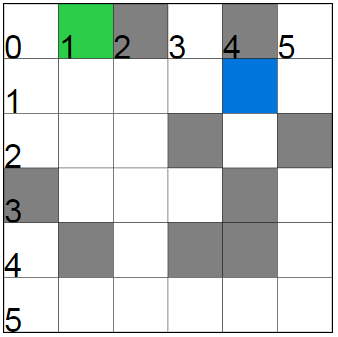
\includegraphics[width=2.10417in,height=2.09722in]{media/image1.png} &
Schreibt Startpunkt in Bekannte Liste mit Distanz Wert. & (4/1) d = 4 &
-\tabularnewline
\begin{minipage}[t]{0.22\columnwidth}\raggedright
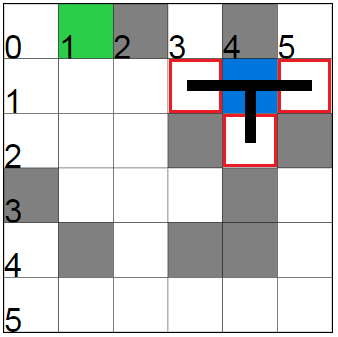
\includegraphics[width=2.10417in,height=2.09722in]{media/image2.png}\strut
\end{minipage} & \begin{minipage}[t]{0.22\columnwidth}\raggedright
Berechne Distanz Wert aller Nachbarn(Rot markiert) und schreibe diese in
die bekannte Knoten-Liste. Verweise auf den Vorgängigen Knoten(Schwarzer
Balken).Da (4/1) Alle bekannte Nachbarn hat, wird dieser Knoten in die
untersuchten Knoten-Liste verschoben. Der Knopf mit den tiefsten d Wert
wird Angeschaut und der Prozess wird wiederholt.\strut
\end{minipage} & \begin{minipage}[t]{0.22\columnwidth}\raggedright
(3/1) d = 3

(5/1) d = 5

(4/2) d = 5\strut
\end{minipage} & \begin{minipage}[t]{0.22\columnwidth}\raggedright
(4/1) d = 4\strut
\end{minipage}\tabularnewline
\begin{minipage}[t]{0.22\columnwidth}\raggedright
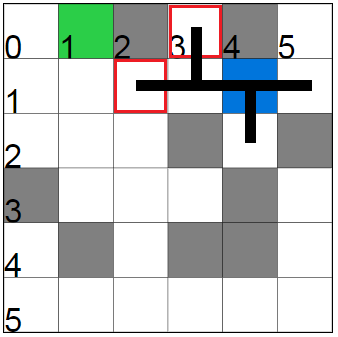
\includegraphics[width=2.10417in,height=2.09722in]{media/image3.png}\strut
\end{minipage} & \begin{minipage}[t]{0.22\columnwidth}\raggedright
Da der Graph(3/1) Alle bekannten Nachbarn hat, wird dieser Knoten in der
untersuchten Knoten-Liste verschoben.\strut
\end{minipage} & \begin{minipage}[t]{0.22\columnwidth}\raggedright
(3/0) d = 2

(2/1) d = 2

(5/1) d = 5

(4/2) d = 5\strut
\end{minipage} & \begin{minipage}[t]{0.22\columnwidth}\raggedright
(3/1) d = 3

(4/1) d = 4\strut
\end{minipage}\tabularnewline
\begin{minipage}[t]{0.22\columnwidth}\raggedright
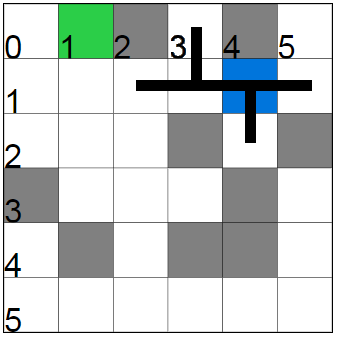
\includegraphics[width=2.10417in,height=2.09722in]{media/image4.png}\strut
\end{minipage} & \begin{minipage}[t]{0.22\columnwidth}\raggedright
Falls Graph(3/0) vor Graph(2/1) angeschaut wird(gleiche d Werte), wird
dieser, da er keine gültigen Nachbarn hat, in die untersuchten
Knoten-Liste geschrieben.\strut
\end{minipage} & \begin{minipage}[t]{0.22\columnwidth}\raggedright
(2/1) d = 2

(5/1) d = 5

(4/2) d = 5\strut
\end{minipage} & \begin{minipage}[t]{0.22\columnwidth}\raggedright
(3/0) d = 2

(3/1) d = 3

(4/1) d = 4\strut
\end{minipage}\tabularnewline
\begin{minipage}[t]{0.22\columnwidth}\raggedright
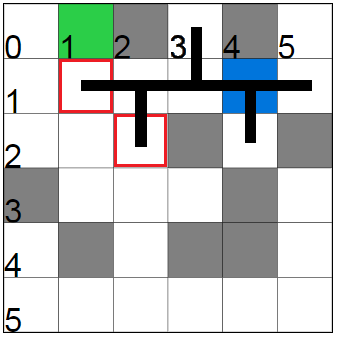
\includegraphics[width=2.10417in,height=2.09722in]{media/image5.png}\strut
\end{minipage} & \begin{minipage}[t]{0.22\columnwidth}\raggedright
Der Prozess wird weitergeführt. Die Listen werden kontinuierlich
aktualisiert.\strut
\end{minipage} & \begin{minipage}[t]{0.22\columnwidth}\raggedright
(1/1) d = 1

(2/2) d = 2

(3/1) d = 3

(5/1) d = 5

(4/2) d = 5\strut
\end{minipage} & \begin{minipage}[t]{0.22\columnwidth}\raggedright
(3/0) d = 2

(2/1) d = 2

(4/1) d = 4\strut
\end{minipage}\tabularnewline
\begin{minipage}[t]{0.22\columnwidth}\raggedright
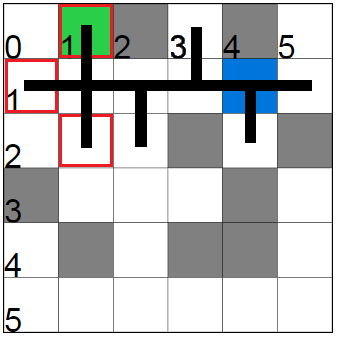
\includegraphics[width=2.10417in,height=2.09722in]{media/image6.png}\strut
\end{minipage} & \begin{minipage}[t]{0.22\columnwidth}\raggedright
Der A-Star hat das Ziel erreicht und muss noch den einzelnen Graphen
zurück folgen bis zum Start und kennt somit den Weg.\strut
\end{minipage} & \begin{minipage}[t]{0.22\columnwidth}\raggedright
(1/0) d = 0

(0/1) d = 2

(1/2) d = 2

(2/2) d = 2

(3/1) d = 3

(5/1) d = 5

(4/2) d = 5\strut
\end{minipage} & \begin{minipage}[t]{0.22\columnwidth}\raggedright
(1/1) d = 1

(3/0) d = 2

(2/1) d = 2

(4/1) d = 4\strut
\end{minipage}\tabularnewline
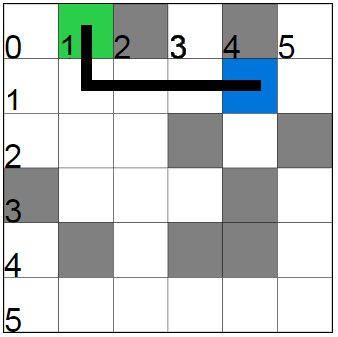
\includegraphics[width=2.10417in,height=2.09722in]{media/image7.png} &
Die Suche ist Beendet. & - & -\tabularnewline
\bottomrule
\end{longtable}

\textbf{BestFirstFinder}

Wie der Name schon sagt sucht dieser Pathfind-Algorithmus nach dem
erstbesten Weg zum Ziel. Im Vergleich zum A-Star hat dieser bloss eine
Liste mit offenen Knoten. Mit der Manhattan Heuristik wird nur der Weg
zum tiefsten Distanz wert Graph in diese Liste eingetragen, somit schaut
der Bestfirstfinder nicht auf alle nachbarknoten.

\textbf{Funktionsweise}

Es wird eine Liste für die Offenen Knoten eröffnet und der Startknoten
wird eingetragen. Auch hier verweist jeder Knoten auf seinen Vorgänger.
Der beste Knoten aus der Liste wird n genannt. Schau die Nachbarn von n
an und bewerte diese mit der Heuristik, der beste Wert wird in die Liste
eingetragen und der Ablauf wird wiederholt. Kommt ein Knoten, der
angeschaut wird, nicht weiter, wird der zweitbeste Graph in der Liste
Angeschaut. Es kann einer weiten Liste hinzugefügt werden, die
geschlossene Liste, die den Lösungsweg direkt mit Abspeichert und
verhindert, dass dieser Algorithmus nicht in einer Endlosschleife endet.

{[}https://developer.roblox.com/articles/Best-first-search\#Pseudo\_Code{]}

\textbf{Beispiel}

Blau ist Startpunkt und Grün Zielpunkt, Diagonale Verbindungen sind
nicht verfügbar.

\begin{longtable}[]{@{}lll@{}}
\toprule
\endhead
Bild & Ausführung & Liste\tabularnewline
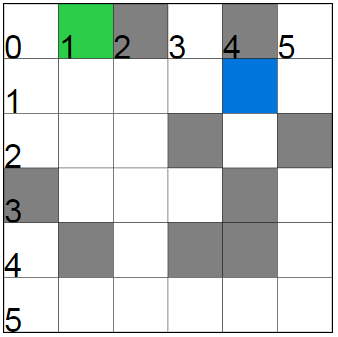
\includegraphics[width=1.9375in,height=1.93056in]{media/image1.png} &
Schreibe Startpunkt in die Liste. & (4/1) d = 4\tabularnewline
\begin{minipage}[t]{0.30\columnwidth}\raggedright
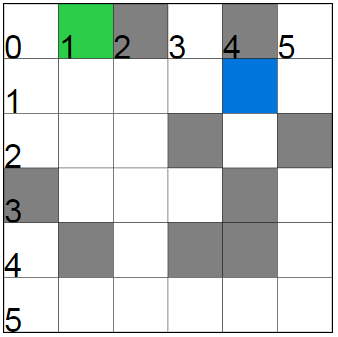
\includegraphics[width=1.9375in,height=1.93056in]{media/image8.png}\strut
\end{minipage} & \begin{minipage}[t]{0.30\columnwidth}\raggedright
Wähle den besten Nachbar, anhand seiner Distanz Wert d, hier ist es
Graph(3/1). Schreibe diesen Wert in die Liste.\strut
\end{minipage} & \begin{minipage}[t]{0.30\columnwidth}\raggedright
(3/1) d = 3

(4/1) d = 4\strut
\end{minipage}\tabularnewline
\begin{minipage}[t]{0.30\columnwidth}\raggedright
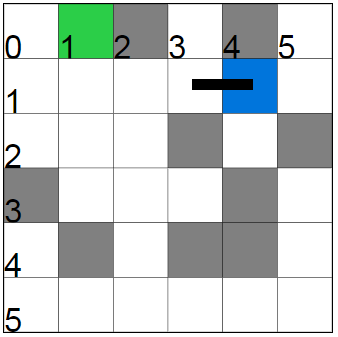
\includegraphics[width=1.9375in,height=1.93056in]{media/image9.png}\strut
\end{minipage} & \begin{minipage}[t]{0.30\columnwidth}\raggedright
Wiederhole die Ausführung bis das Ziel erreicht wurde.\strut
\end{minipage} & \begin{minipage}[t]{0.30\columnwidth}\raggedright
(2/1) d = 2

(3/1) d = 3

(4/1) d = 4\strut
\end{minipage}\tabularnewline
\begin{minipage}[t]{0.30\columnwidth}\raggedright
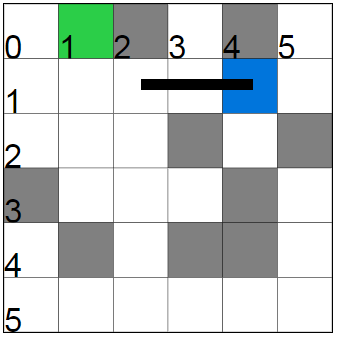
\includegraphics[width=1.9375in,height=1.93056in]{media/image10.png}\strut
\end{minipage} & \begin{minipage}[t]{0.30\columnwidth}\raggedright
\strut
\end{minipage} & \begin{minipage}[t]{0.30\columnwidth}\raggedright
(1/1) d = 1

(2/1) d = 2

(3/1) d = 3

(4/1) d = 4\strut
\end{minipage}\tabularnewline
\begin{minipage}[t]{0.30\columnwidth}\raggedright
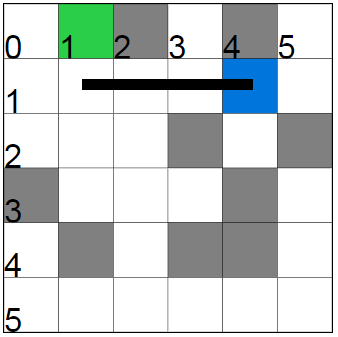
\includegraphics[width=1.9375in,height=1.93056in]{media/image11.png}\strut
\end{minipage} & \begin{minipage}[t]{0.30\columnwidth}\raggedright
Der Weg wurde gefunden\strut
\end{minipage} & \begin{minipage}[t]{0.30\columnwidth}\raggedright
(1/0) d = 0

(1/1) d = 1

(2/1) d = 2

(3/1) d = 3

(4/1) d = 4\strut
\end{minipage}\tabularnewline
\bottomrule
\end{longtable}

\textbf{BreadthFirstFinder}

Der BreadthFirstFinder benutzt keine Heuristik, da er sein Weg über die
Breitensuche findet. Er Expandiert in jede Richtung gleich schnell und
bewegt sich nicht wie die anderen zwei Pathfinder in Richtung Ziel. Wenn
alle Knoten mit der gleichen Distanz zum Start angeschaut sind, beginnt
er mit der Suche der eins weiter entfernten Knoten. Dieser Pathfinder
besitzt eine Liste in der er die noch zu bearbeitenden Knoten speichert,
beginnend mit dem am Start nächsten Knoten.

{[}https://brilliant.org/wiki/breadth-first-search-bfs/{]}

\textbf{Funktionsweise}

Beginne beim Startpunkt und Speichere ihn in die Warteliste. Schaue am
obersten Knoten in der Warteschlange dessen Nachbarn an und prüfe ob
eines der Ausgewählten Knoten der Zielknoten ist. Ist dies der Fall wird
die Suche Abgebrochen, da der Weg Gefunden wurde. Falls keiner der
Knoten der Zielknoten ist, speichere die neuen Knoten in die Warteliste
an Hinterste Stelle und entferne den Ausgewählten Knoten. Jeder Knote
der neu gefunden wird zeigt auf den ausgewählten Knoten.

{[}https://brilliant.org/wiki/breadth-first-search-bfs/{]}

\textbf{Beispiel}

Blau ist Startpunkt und Grün Zielpunkt, Diagonale Verbindungen sind
nicht verfügbar.

\begin{longtable}[]{@{}lll@{}}
\toprule
\endhead
\textbf{Bild} & \textbf{Ausführung} & \textbf{Liste}\tabularnewline
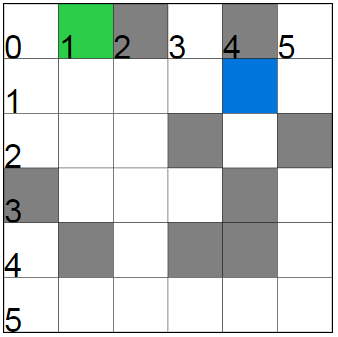
\includegraphics[width=1.9375in,height=1.93056in]{media/image1.png} &
Schreibe den Startpunkt in die Liste. & (4/1)\tabularnewline
\begin{minipage}[t]{0.30\columnwidth}\raggedright
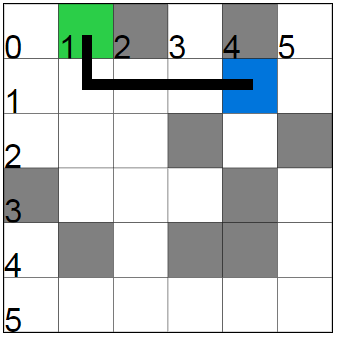
\includegraphics[width=1.9375in,height=1.93056in]{media/image12.png}\strut
\end{minipage} & \begin{minipage}[t]{0.30\columnwidth}\raggedright
Schaue alle Nachbarn an und speichere diese in die Liste an hinterste
Stelle. Falls keiner der neuen Knoten das Ziel ist, führe suche fort.
Jeder neue Graph verweist auf den Vorgänger. Entferne aktuellen
ausgewählten Knoten(4/1).\strut
\end{minipage} & \begin{minipage}[t]{0.30\columnwidth}\raggedright
(3/1)

(5/1)

(2/1)\strut
\end{minipage}\tabularnewline
\begin{minipage}[t]{0.30\columnwidth}\raggedright
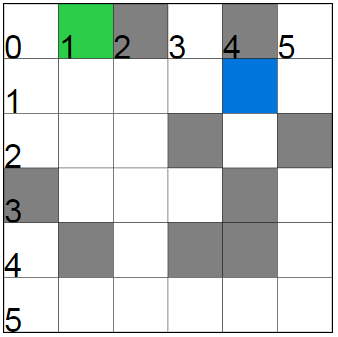
\includegraphics[width=1.9375in,height=1.93056in]{media/image13.png}\strut
\end{minipage} & \begin{minipage}[t]{0.30\columnwidth}\raggedright
Schaue alle Nachbarn der zurzeit in der Liste stehenden Knoten und
Wiederhole alles vom oben genannte.\strut
\end{minipage} & \begin{minipage}[t]{0.30\columnwidth}\raggedright
(3/1)

(2/1)

(5/1)\strut
\end{minipage}\tabularnewline
\begin{minipage}[t]{0.30\columnwidth}\raggedright
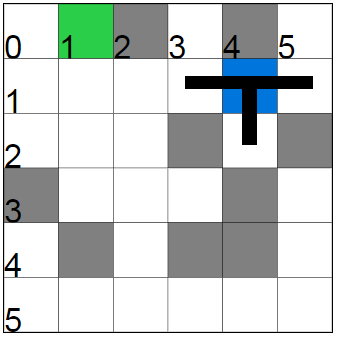
\includegraphics[width=1.9375in,height=1.93056in]{media/image14.png}\strut
\end{minipage} & \begin{minipage}[t]{0.30\columnwidth}\raggedright
\strut
\end{minipage} & \begin{minipage}[t]{0.30\columnwidth}\raggedright
(1/1)

(2/2)\strut
\end{minipage}\tabularnewline
\begin{minipage}[t]{0.30\columnwidth}\raggedright
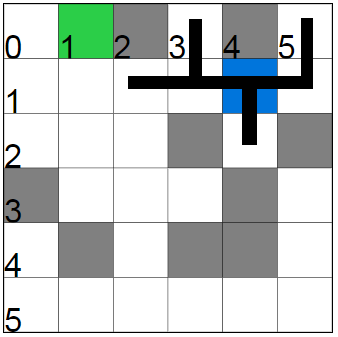
\includegraphics[width=1.9375in,height=1.93056in]{media/image15.png}\strut
\end{minipage} & \begin{minipage}[t]{0.30\columnwidth}\raggedright
Das Ziel Wurde Gefunden und die Suche kann beendet werden. Folgen vom
Ziel zum Start und gib den Lösungsweg aus.\strut
\end{minipage} & \begin{minipage}[t]{0.30\columnwidth}\raggedright
(0/1)

(1/0)

(1/2)

(2/3)\strut
\end{minipage}\tabularnewline
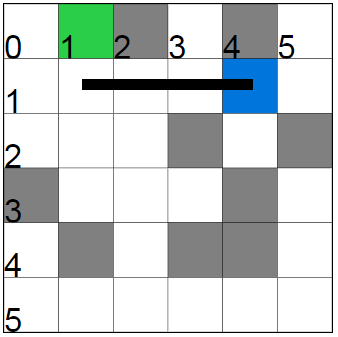
\includegraphics[width=1.9375in,height=1.93056in]{media/image11.png} &
Lösung & -\tabularnewline
\bottomrule
\end{longtable}

\textbf{Vor- und Nachteile der einzelnen Pathfinder}

Anhand der Beispiele am gleichen Raster sieht man sehr gut, dass alle
drei Pathfinder den gleichen Weg finden durch unterschiedliche Methoden.

Der A-Star führt viele Heuristik Berechnungen durch, da er von jedem
Knoten die Distanz zum Ziel speichern möchte. Dies erfordert mehr
Rechenleistung beziehungsweise mehr Operationen als die beiden anderen.
Bei Komplexeren Raste wird er jedoch immer den besseren Weg finden.

Der BestFirstFinder untersucht nur den zuerst gefunden besten Weg und
sucht daher zuerst in der tiefe. Er braucht weniger Rechenleistung als
der A-Star, kann aber mühe bekommen, falls der erst gesuchte Weg in eine
Sackgasse führt. In diesem Beispiel musste er weniger Knoten anschauen
als der A-Star, obwohl er die gleiche Heuristik benutzt.

Der BreadthFirstFinder suche alle ihm am nächsten gelegenen Knoten ab
und wird immer auf eine Lösung kommen auf Kosten der ``unnötigen''
Knoten die weiter entfernt zum Ziel als seine aktuelle Position. Die
Warteliste wird mit jeder neuen Expansion um ein vielfaches grösser und
die Expansion Erweiterung wird über die Dauer langsamer.
%%%%%%%%%%%%%%%%%%%%%%%%%%%%%%%%%%%%%%%%%%%%%%%%%%%%%%%%%%%%%%%%%%%%%%
\textbf{Realisierung der Webapplikation}

\textbf{@@@@@}

\textbf{Vergleiche der Algorithmen / Statistik }

Alle Notierten Messresultate pro Vergleich befinden sich im Anhang
dieser Arbeit.

Das Autorenteam hat sich auf eine Rastergrösse von 50x50 Felder
entschieden und durchlief die Vergleiche 125-mal. Die Rechenzeit wurde
auf 0.1ms gerundet. Die Diagonalen wurden mitbeachtet, da dies zu
Optimierten Strecken führen kann.

Diese 125 Versuche wurden zuerst in folgende Kategorien in den Resultate
unterteilt: Weg des kürzesten patinier von 0-10 Felder, 11-20 Felder,
21-30 Felder, 31-40 Felder, 41-50 Felder. Jede dieser Unterteilung hat
25 Vergleich Ergebnisse. Diese Unterteilung hat den Grund, dass auf
längeren Wege die Unterschiede nach der Erfahrung dieser Arbeit durch
das Autorenteam besser zu sehen sind.

\begin{longtable}[]{@{}l@{}}
\toprule
\endhead
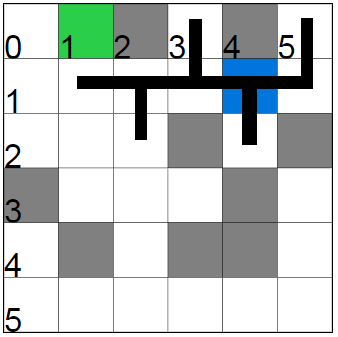
\includegraphics[width=6.26111in,height=4.02639in]{media/image16.jpeg}\tabularnewline
\bottomrule
\end{longtable}

Man erkennt gut, dass der A-Star und BreadthFirstFinder ca. die gleiche
Felder Distanz Finden. Je Grösser der Abstand von Start und Ziel in
Feldern, desto grösser ist der Unterschied zwischen dem BestFirtFinder
und den anderen zwei.

\begin{longtable}[]{@{}l@{}}
\toprule
\endhead
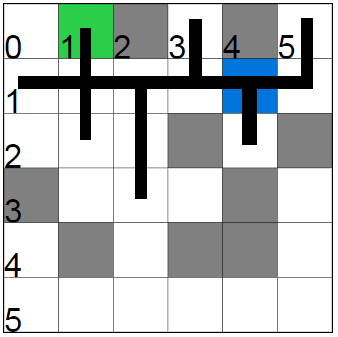
\includegraphics[width=6.26111in,height=3.95625in]{media/image17.jpeg}\tabularnewline
\bottomrule
\end{longtable}

Man beachte, die Diagramm-Darstellung ist Logarithmisch. Im Aufwand der
ausgeführten Operationen steigt der BreadthFirstFinder viel extremer als
die anderen. Der A-Star muss im Verhältnis zum BestFirstFinder immer
mehr Operationen Ausführen. Die Steigung des BreadthFirstFinder senkt
sich im Laufe der Felder Distanz, dies kommt daher, dass er am Rand des
Rasters ist und diese Seite nicht mehr weiter erkunden muss. Die
Vorteile einer Heuristik wird hier klar verdeutlicht, der A-Star und
BestFirstFinder müssen durch die Wahrscheinlichkeit Berechnung weniger
Operationen durchlaufen.

\begin{longtable}[]{@{}l@{}}
\toprule
\endhead
\includegraphics[width=6.26944in,height=4.15625in]{media/image18.jpeg}\tabularnewline
\bottomrule
\end{longtable}

Da der BestFirstFinder den erst besten Weg tiefer durchsucht, ist seine
Rechen Zeit um einiges verkürzt als die Anderen. Da der
BreadthFirstFinder am meisten Operationen hat, ist es logisch, dass
seine Rechen Zeit höher als A-Star oder BestFirstFinder ist.

\textbf{Interpretation Resultate}

Durch die Statistik Diagramme kann man folgendes herauslesen:

\begin{itemize}
\item
  Der A-Star und BreadthFirstFinder finden ca. den gleich optimalen Weg,
  wobei der BreadthFirstFinder viel mehr an Operationen aufwenden muss,
  da er keine Heuristik besitzt.
\item
  Hat man begrenzte Zeit, so ist der BestFirstFinder gut geeignet, er
  findet nicht den Optimalsten Weg, spart dafür in Zeit und Operationen.
\item
  Je grösser das Raster, desto weniger ist der BreadthFirstFinder
  geeignet, da er zu viele Operationen benötigt und langsam wird im
  Vergleich zum A-Star.
\item
  Die Rechenzeit vom BestFirstFinder steigt linear, die Rechenzeit vom
  A-Star und BreadthFirstFinder exponential solange der
  BreadthFirstFinder keine Rasterseite erreicht hat.
\end{itemize}

\textbf{Schluss}

\textbf{Quellenverzeichnis}

\textbf{Dank}

\textbf{Anhang}

\textbf{Bescheinigung}
